\documentclass{article}

% if you need to pass options to natbib, use, e.g.:
%     \PassOptionsToPackage{numbers, compress}{natbib}
% before loading neurips_2018

% ready for submission
% \usepackage{neurips_2018}

% to compile a preprint version, e.g., for submission to arXiv, add add the
% [preprint] option:
 % \usepackage[preprint]{neurips_2018}

% to compile a camera-ready version, add the [final] option, e.g.:
 \usepackage[final]{neurips_2019}
% to avoid loading the natbib package, add option nonatbib:
%     \usepackage[nonatbib]{neurips_2018}
\usepackage{graphicx}
\usepackage[utf8]{inputenc} % allow utf-8 input
\usepackage[T1]{fontenc}    % use 8-bit T1 fonts
\usepackage{hyperref}       % hyperlinks
\usepackage{url}            % simple URL typesetting
\usepackage{booktabs}       % professional-quality tables
\usepackage{amsfonts}       % blackboard math symbols
\usepackage{nicefrac}       % compact symbols for 1/2, etc.
\usepackage{microtype}      % microtypography
\usepackage{amsmath}
\usepackage{bm}
\usepackage{subfig}
\usepackage[english]{babel}
\usepackage{algorithm}
\usepackage{algorithmic}
\usepackage{appendix}
\newtheorem{theorem}{Theorem}
\newtheorem{lemma}{Lemma}
\newtheorem{exam}{Example}
\newtheorem{proof}{Proof}
\input macros.tex

\newcommand*{\KeepStyleUnderBrace}[1]{%f
  \mathop{%
    \mathchoice
    {\underbrace{\displaystyle#1}}%
    {\underbrace{\textstyle#1}}%
    {\underbrace{\scriptstyle#1}}%
    {\underbrace{\scriptscriptstyle#1}}%
  }\limits
}
\usepackage{xr}
\externaldocument{nips_2019_miaoyan}

\title{Supplements for ``Multi-way clustering via tensor block models''}


%\author{%
%Yuchen Zeng \\
%University of Wisconsin -- Madison\\
 %\texttt{yzeng58@wisc.edu} \\
%\And
%Miaoyan Wang \\
%University of Wisconsin -- Madison\\
%\texttt{miaoyan.wang@wisc.edu} \\
%}

\begin{document}

\maketitle

\vspace{-2cm}
\begin{appendices}
\section{Proofs}
	
\subsection{Proof of Proposition~\ref{prop:factors}}
Let $\tS=\{\mathbb{P}_{\Theta}\colon \Theta\in\tP\}$ be the family of (either Gaussian or Bernoulli) tensor block models~\eqref{eq:Tucker}, where $\Theta=\tC \times_1\mM_1\times_2\cdots\times_K\mM_K$ parameterizes the mean block tensor. Since the mapping $\Theta\mapsto\mathbb{P}_{\Theta}$ is one-to-one, $\Theta$ is identifiable. Now suppose there are two decompositions of $\Theta=\Theta(\{\mM_k\}, \tC)=\Theta(\{\tilde \mM_k\}, \tilde \tC)$. Based on the Assumption~\ref{ass:core}, we have
\begin{equation}\label{eq:equality}
\Theta=\tC \times_1\mM_1\times_2\cdots\times_K\mM_K=\tilde \tC \times_1\tilde \mM_1\times_2\cdots\times_K\tilde  \mM_K,
\end{equation}
where $\tC$, $\tilde \tC\in\mathbb{R}^{R_1\times \cdots \times R_K}$ are two irreducible cores, and $\mM_k,\tilde \mM_k\in\{0,1\}^{R_k\times d_k}$ are membership matrices for all $k\in[K]$. We will prove by contradiction that $\mM_k$ and $\tilde \mM_k$ induce the same partition of $[d_k]$, for all $k\in[K]$. 

Suppose the above claim does not hold. Then there exists a mode $k\in[K]$ such that the $\mM_k, \tilde \mM_k$ induce two different partitions of $[d_k]$. Without loss of generality, we assume $k=1$. The definition of partition implies that there exists a pair of indices $i\neq j, i,j\in[d_1]$, such that, $i,j$ belong to the same cluster based on $\mM_k$, but they belong to different clusters based on $\tilde \mM_k$. Let $\tC\subset [d_1] $ denote the cluster that $i$ (or $j$) belong to based on $\mM_k$, and $\tA, \tB\subset[d_1]$ denote the two different clusters that $i$, $j$ belongs to based on $\tilde \mM_k$. Based on the left-hand side of \eqref{eq:equality}
\begin{equation}\label{eq:cluster1}
\Theta_{i,i_2,\ldots,i_K}=\Theta_{j,i_2,\ldots,i_K},\quad \text{for all } (i_2,\ldots,i_K)\in[d_2]\times\cdots\times [d_K].
\end{equation}
 On the other hand, \eqref{eq:equality} implies
\begin{equation}\label{eq:cluster2}
\Theta_{i,i_2,\ldots,i_K}=\Theta_{k,i_2,\ldots,i_K},\quad \text{for all } k\in \tA \text{ and }(i_2,\ldots,i_K)\in[d_2]\times\cdots\times [d_K],
\end{equation}
and
\begin{equation}\label{eq:cluster3}
\Theta_{j,i_2,\ldots,i_K}=\Theta_{k,i_2,\ldots,i_K},\quad \text{for all } k\in \tB \text{ and }(i_2,\ldots,i_K)\in[d_2]\times\cdots\times [d_K].
\end{equation}

Combining~\eqref{eq:cluster1}, \eqref{eq:cluster2} and \eqref{eq:cluster3}, we have
\[
\Theta{i,i_2,\ldots,i_K}=\Theta_{k,i_2,\ldots,i_K},\quad \text{for all } k\in \tA\cup \tB \text{ and }(i_2,\ldots,i_K)\in[d_2]\times\cdots\times [d_K].
\]
Therefore, one can merge $\tA, \tB$ into one cluster along the mode 1. This contradicts the irreducibility of the core tensor $\tilde \tC$. Therefore, $\mM_1$ and $\tilde \mM_1$ induce a same partition of $[d_1]$, and thus they are equal up to permutations. The proof is now complete. 


%Based on the definition of membership matrix, $\mM_k\mM_k'=\text{diag}(R_1,\ldots,R_K)$ is a diagonal matrix and thus invertible. Multiplying $\mM_k'(\mM_k\mM_k')^{-1}$ to the $k$-th mode of Equation~\eqref{eq:equality} gives
%\begin{equation}\label{eq:core}
%\tC=\tilde \tC \times_1\left(\tilde \mM_1 \mM_1'(\mM_1\mM_1')^{-1}\right) \times_2\cdots\times_K \left(\tilde   \mM_K \mM_K'(\mM_K\mM_K')^{-1}\right).
%\end{equation}
%Define $\mB_k=\tilde \mM_k \mM_k'(\mM_k\mM_k')^{-1}$. It remains to show that each $\mB_k$ is a permutation matrix. 


%Now, the definition of membership matrix implies that $\mB_k$ is a column-wise normalized confusion matrix, where its $(r,s)$-th entry is
%\[
%\mB_{k,(r,s)}={ \#\{i\in[d]: \tilde \mM_k(i)=r, \mM_k(i)=s\}\over \#\{i\in[d]: \mM_k(i)=s\}}\in[0,1],
%\] 
%where $\#$ denotes the cardinality size of the set. Plugging $\mB_k$ back to the Equations~\eqref{eq:equality} and~\eqref{eq:core} yields
%\begin{equation}\label{eq:cluster}
%\tilde \tC \times_1 \left(\mB_1\mM_1\right) \times_2 \cdots\times_K \left(\mB_K\mM_K\right)=\tilde \tC \times_1 \tilde \mM_1 \times_2 \cdots\times_K \tilde \mM_K.
%\end{equation}
%Both sides of the above expression represent a block tensor with a same core. Let us consider the mode-1 structure first. Based on the Assumption~\ref{ass:core}, $\mB_1\mM_1$ has full row rank. Furthermore, the mode-$1$ partition is determined by $\mM_1$, because multiplying a $R_1$-by-$R_1$ confusion matrix $B_1$ will not change the cluster allocation. On the right-hand hand, the mode-$1$ partition is determined by $\tilde \mM_1$. Therefore the partition encoded in $\mM_1$ is the same as that in $\tilde \mM_1$. Equivalently, $\mB_1$ must be a permutation matrix. The proof is complete by applying the same argument to all $k\in[K]$. 
%\subsection{Proof of Theorem~\ref{thm:main}}
%We first present three lemmas that will be used in the proof of Theorem~\ref{thm:main}. 
%\begin{lemma} 
%\end{lemma}

\subsection{Proof of Theorem~\ref{thm:main}}
To study the performance of the least-square estimator $\hat \Theta$, we need to introduce some additional notations. We view the membership matrix $\mM_k$ as an onto function $\mM_k\colon [d_k]\mapsto [R_k]$, and with a little abuse of notation, we still use $\mM_k$ to denote the mapping function. Correspondingly, we use $\mM_k(i_k)$ to denote the cluster label for the element $i_k\in[d_k]$, and $\mM^{-1}_k(r_k)$ the group of elements in cluster $r_k\in[R_k]$.

To simplify notation, we define $\mi=(i_1,\ldots,i_K)$, $\mr=(r_1,\ldots,r_K)$, and $\mM^{-1}(\mi)=\mM_1^{-1}(r_1)\times \cdots \times \mM^{-1}_K(r_K)$. 
The parameter space $\tP$ can be equivalently written as
\begin{align}
\tP=&\big\{ \Theta\in\mathbb{R}^{d_1\times \cdots\times d_K}\colon \Theta_{\mi}=\tC_{\mr} \text{ for }\mi \in\mM^{-1}(\mr)\text{ and a core tensor $\tC\in\mathbb{R}^{R_1\times \cdots \times R_K}$} \big\}.\notag
\end{align}
That is, the mean signal tensor $\Theta$ is a piecewise constant with respect to the blocks in the Cartesian product of the mode-$k$ clusters, $\mM^{-1}(\mi)$, for all $\mr \in[R_1]\times \cdots\times [R_K]$. 

The estimate $\hat \Theta$ consists of two components: the mean parameter $\tC$ and the clustering (structure) parameter $ \mM\colon [d_1]\times \cdots [d_K]\mapsto [R_1]\times \cdots \times [R_K]$. We introduce an intermediate estimate 
\[
\bar \Theta =\mathbb{E}(\hat \Theta|\hat \mM)=\mathbb{E}(\hat \tC\times_1 \hat \mM_1\times\cdots \times_K \hat \mM_K|\hat \mM),
\] 
where the expectation is taken with respect to the $\hat \tC$ (which is a function of the data $\tY$). Note that, given the structure estimate $\hat \mM$, the mean estimate $\hat \tC$ is simply the sample average of $\tY$ within the blocks defined by $\hat \mM$. Therefore, 
%\begin{align}
%\bar \Theta=\mathbb{E}(\hat \tC|\hat \mM)\times_1\hat \mM_1\times\cdots \times_k \hat \mM_K&=\tC\times_1 (\mB_1\hat \mM_1)\cdots \times_K(\mB_K\hat \mM_K)\\
%&=\KeepStyleUnderBrace{(\tC\times_1\mB_1\times \cdots \times_K \mB_K)}_{\bar \tC}\times_1\hat \mM_1\times_2 \cdots \times_K\hat \mM_K
%\end{align}
%where $\mB_k=\mM_k\hat \mM'_k(\hat \mM_k\hat \mM'_k)^{-1}$ is the (row-normalized) confusion matrix between $\mM_k$ and $\mM'_k$, for all $k\in[K]$.
Note that $\hat \Theta$ is the minimizer of $\FnormSize{}{\Theta -\tY}$. By Lemma 1, 
\[
\FnormSize{}{\hat \Theta -\trueT}\leq 2 \langle \hat \Theta-\bar\Theta,\ \tY-\trueT \rangle+2\FnormSize{}{\hat \Theta-\bar\Theta} \delta +2 \delta^2
\]
where $\delta=|\langle {\bar \Theta -\trueT\over  \FnormSize{}{\bar \Theta-\trueT}}, \tY-\trueT  \rangle|.$

\begin{lemma} With probability at least $1-\exp(\prod_k R_k + \sum_k d_k \log R_k)$
\[
\langle\hat \Theta -\bar \Theta, \tY-\trueT\rangle\leq C_1\sigma^2 \left( \prod_k R_k+\sum_k R_k\log d_K\right),
\]
holds uniformly over $\hat \mM$. 
\end{lemma}

\begin{proof}
 For any fixed index $\mi\in[d_1]\times \cdots [d_K]$. Suppose that the index $\mi$ belongs to the block $\mr$ according to $\hat \mM$; i.e. $\hat \mM(\mi)=\mr$. Then
\[
\hat \Theta_{\mi}={1\over |\hat \mM^{-1}(\mr)|} \sum_{\mj\in\hat \mM^{-1}(\mr)}\tY_{\mj}.
\]
By the definition of $\bar \Theta=\mathbb{E}(\hat \Theta|\hat \mM)$, we have
\begin{align}
\hat \Theta_{\mi}-\bar \Theta_{\mi}&={1\over |\hat \mM^{-1}(\mr)|} \sum_{\mj\in\hat \mM^{-1}(\mr)}\left(\tY_{\mj}-\mathbb{E}(\tY_{\mj})\right)\\
&={1\over| \hat \mM^{-1}(\mr)|} \sum_{\mj\in\hat \mM^{-1}(\mr)}\tE_{\mj}
\end{align}
Therefore, 
\[
\langle \hat \Theta-\bar \Theta, \tY-\trueT\rangle=\sum_{\mr}\left({1\over \sqrt{|\hat \mM^{-1}(\mr)|}} \sum_{\mj\in\hat \mM^{-1}(\mr)}\tE_{\mj}\right)^2
\]
Note that $\tE_{\mj}$ follows the independent sub-Gaussian-$\sigma^2$ assumption. Hence
\[
{1\over \sqrt{|\hat \mM^{-1}(\mr)|}} \sum_{\mj\in\hat \mM^{-1}(\mr)}\tE_{\mj}
\]
follows sub-Gaussian with-$\sigma^2$. There are $\prod_k R_k$ choices of $\mr$. By union bound, with probability at least $1-\exp(\prod_k R_k+\sum_k d_k\log R_k)$
\[
|\hat \Theta-\bar\Theta, \tY-\trueT| \leq C_1 \sigma^2 \left(\prod_k R_k+\sum_k d_k \log R_k\right)
\]
uniformly holds for all $\hat \mM$.
\end{proof}
\begin{lemma} With probability at least $1-\exp(\sum_k d_k \log R_k)$,
\[
\Big \langle{ \bar \Theta -\trueT \over \FnormSize{}{\bar \Theta -\trueT}},\ \tY-\trueT \Big \rangle\leq C_2\sigma\left(\prod_k d_k+\sum_k d_k \log R_k \right)^{1/2}.
\]
\end{lemma}
\begin{proof}
Define 
\[
\tB=\{ \entry{\tC}: \}
\]
\end{proof}

\begin{lemma} With probability at least $1-\exp(\sum_k R_k+\sum_k R_k\log d_k)$,
\[
\FnormSize{}{\hat \Theta -\bar \Theta}\leq C_3\sigma\left(\prod_k R_k+\sum_k d_k \log R_k \right)^{1/2}.
\]
\end{lemma}

\begin{proof} From the proof of Lemma 1, we have
\[
\FnormSize{}{\hat \Theta-\bar \Theta}^2=\sum_{\mr}{1\over |\mM^{-1}(\mr)|}\left(\sum_{\mj \in \hat \mM^{-1}(\mr)}\tE_{\mj}\right)^2.
\]
Note that ${{1\over \sqrt{|\mM^{-1}(\mr)|}}\sum_{\mj\in \hat \mM^{-1}(\mr)}\tE_{\mj}$ follows independent Gaussian-$\sigma$. (same as Lemma 1?) So
\[
\FnormSize{}{\hat \Theta-\bar \Theta} \leq C \sigma\left(\prod_k R_k+\sum_k d_k \log R_k\right)
\]
uniformly over $\mM$.
\end{proof}

\begin{lemma} Let $\ma, \mb\in\mathbb{R}^d$ be two vectors and $\normSize{}{\cdot}$ the Euclidean norm in $\mathbb{R}^2$. If $\normSize{}{\mb}\leq \normSize{}{\ma}$, then the following hold for any $\mx\in\mathbb{R}^d$:
\[
\normSize{}{\ma-\mb}\leq 2 \langle \mx,\ma\rangle  + 2\normSize{}{\mx}\delta+2\delta^2,\quad \text{with}\quad \delta=\Big|\large \Big\langle{\ma-\mb-\mx\over\normSize{}{\ma-\mb-\mx}},\ \ma \Big\rangle\Big|
\]
\end{lemma}
Let $d=\prod_k d_k$ and $R=\prod_k R_k$. We define $\tD(s)$ to be the set of $d$-dimensional vectors with at most $s$ distinct entry values. 
By identifying the tensors in $\tP$ as $d$-dimensional vectors, we have $\tP\subset \tD^d(R)$.


Now consider the least-estimate estimator
\[
\hat \Theta=\argmin_{\Theta\in\tP}\{-2\langle \tY, \Theta\rangle+\FnormSize{}{\Theta}^2 \}=\argmin_{\Theta\in\tP}\{\FnormSize{}{\tY-\Theta}^2 \}.
\]
Based on Proposition~\ref{prop:bound}, we have
\[
\FnormSize{}{\hat \Theta-\trueT} \leq 2\sup_{\mu\in (\tP-\tP') \cap \mB^d_2}\langle \mu ,\tE\rangle,
\]
where $(\tP-\tP')=\{\mu-\mu'\colon \mu, \mu'\in\tP\}$ and $\mB^{d}_2$ denotes the Euclidean unit ball in dimension $d$. Based on the definition we have
\[
(\tP-\tP')\subset \tD^d(R^2).
\]

(to be finished...)
\begin{align}
\FnormSize{}{\hat \Theta-\trueT}&\leq 2\sup_{\mu\in\tD(R)} \sup_{\mu'\in \tD(R)} \Big\langle {\mu-\mu'\over \FnormSize{}{\mu-\mu'}}, \tE \Big\rangle\\
&\leq \sup_{\mu\in \tD(R)}\sup_{\mu'\in \tD(R)\cap \mB_2(\mu)}\langle \mu', \tE  \rangle\\
&\leq \sup_{\mu \in \tD(R)} 6^R{d \choose R}
\end{align}
\begin{align}
\sup_{\mu\in (\tP-\tP')\cap \mB^d_2}\langle \mu ,\tE\rangle&\leq \sup_{\mu\in \tD()\cap\mB^d_2}\sup_{\tP} \langle \mu, \tE\rangle\\
&\leq \sup_{|\ms|= R^2}\sup_{\mu\in\mB_2^{\ms}}\langle \mu, \tE\rangle\\
&\leq2\sigma \log\left(6^{R^2}{d \choose R^2}\right)\\
&\leq 2\sigma R^2+....
\end{align}
with probability at least $1-\exp(R^2)$

For fixed $\mM_k$'s, $\tC$ is a linear space of dimension no greater than $R^2$. 
%Let $\tD$ denote a subset of $\mathbb{R}$ with $\prod_k R_k$ finite elements. We also call $\tD$ an alphabet with $|\tD|=\prod_k$. Then
%\[
%\tP\subset \{\Theta\colon \Theta\in \tD^{d_1\times \cdots d_K}\}.
%\]

\subsection{Sparse clustering}
\begin{lemma}\label{lem:sparse}
Consider the regularized least-square estimation,
\[
\hat \Theta^{\text{sparse}}=\argmin_{\Theta\in \tP}\left\{\FnormSize{}{\tY-\Theta}^2+\lambda \normSize{}{\tC}_\rho
\right\},
\]
where $\normSize{}{\tC}_\rho$ is the penalty function with $\rho$ being an index for the tensor norm, $\tC=\entry{c_{r_1,\ldots,r_K}}\in\mathbb{R}^{R_1\times \cdots\times R_K}$ is the block means, and $\lambda$ is the penalty tuning parameter. Then we have
\begin{equation}\label{eq:lasso}
\hat c^{\text{sparse}}_{r_1,\ldots,r_K}=
\begin{cases}
\hat c^{\text{ols}}_{r_1,\ldots,r_K}\mathds{1}_{\{|\hat c^{\text{ols}}_{r_1,\ldots,r_K} |\geq {2\sqrt{\lambda} \over \sqrt{n_{r_1,\ldots,r_K}}}\}} & \text{if}\ \rho=1,\\
\text{sign}(\hat c^{\text{ols}}_{r_1,\ldots,r_K})\left( \hat c^{\text{ols}}_{r_1,\ldots,r_K}-{2\lambda \over n_{r_1,\ldots,r_K}}  \right) &\text{if}\ \rho=0.
\end{cases}
\end{equation}
\end{lemma}

\begin{proof}
We cast the problem into a regularized least square. Note that
\[
\Theta=\tC\times_1\mM_1\times \cdots \mM_K.
\]
Let $\mX=\mM_1\otimes \ldots \otimes \mM_K\in \mathbb{R}^{d\times R}$, where $d=\prod_k d_k$ and $R=\prod_k R_k$. The problem is equivalent to a linear regression with $\mY=\text{vec}(\tY)$ as the response and $\mX$ as the design matrix. Note that $\mX$ is an orthogonal matrix with $\mX^T\mX=\text{diag}(n_1,\ldots,n_{R})$, where $n_r$ is the block size. 
Consider the following constrained optimization: 
\begin{equation*}
L=||\mathbf{Y-X}\bm{\beta}||^2_2+\lambda||\bm{\beta}_0||=(\mathbf{Y-X}\bm{\beta})^T(\mathbf{Y-X}\bm{\beta})+\lambda ||\bm{\beta}||_0=L_1+L_2
\end{equation*} 
where $L_1=(\mathbf{Y-X}\bm{\beta})^T(\mathbf{Y-X}\bm{\beta})$, $L_2=\lambda ||\bm{\beta}||_0$. 

	
\textbf{Case 1: $\rho=0$}\par 
The $L_1$ is exactly the $RSS$ in this case. So we compare the increment of $L_1$  when $L_2$ takes different values. We denote $z$ the number of  non-zero elements in $\bm{\beta}$.\\
	(1) Consider the case we have no constraint on $z$. Thus we only have to minimize $L_1$. By the knowledge of linear regression, we know the unique minimizer is $\bm{\hat{\beta}_{ols}}=\mathbf{(X^TX)^{-1}XY}$. Assume there are $m$ zero elements in $\bm{\hat{\beta}_{ols}}$ where $0\leq m \leq p$ \\
	(2) Consider the case we have constraint on $z$: $z = i$, where $i=0,1,2,...,m$. Obviously, among these cases the $L$ can be minimized if and only if $i=m$. So, $z=m$ and $\bm{\hat{\beta}}=\bm{\hat{\beta}_{ols}}$ is the minimizer of $L$ when $0\leq z\leq m$.
	(3) Consider the case that we have constraint on $x$: $z=m+1$. Then we have to take one more non-zero element in $\bm{\beta}$ to be zero. Suppose we take $\hat{\beta}_l \neq 0$ to be 0. Then we obtain 
	\begin{equation*}
		2L_1 -SSE(\beta_1,...,\beta_{l-1},\beta_{l+1},...,\beta_p)=SSR(\beta_l)
	\end{equation*}
	by the columns in $\mathbf{X}$ are orthogonal to each other. Additionally,
	\begin{equation*}
		SSR(\beta_l) = \mathbf{Y}^T(\mathbf{H-H_l})\mathbf{Y} 
	\end{equation*}
	where $\mathbf{H=X(X^TX)^{-1}X}=\sum_{i=1}^p\frac{1}{n_i}\mathbf{x_{(i)}x_{(i)}^T}$, $\mathbf{H_l} = \sum_{i\neq j}\mathbf{x_{(i)}x_{(i)}^T}$, $\hat{\beta}_l = \frac{1}{n_l}\mathbf{x_{l}Y}$. Thus, we can simplify the second equation as:
	\begin{equation*}
		SSR(\beta_l) = n_l\hat{\beta}_l^2
	\end{equation*}
	Thus, by taking $\hat{\beta}_l$ as 0, there is $\frac{n_l\hat{\beta}_l^2}{2}$ increment on $L_1$, $\lambda$ decrement on $L_2$. Obviously, if the increment of $L_1$ is larger than the decrement $L_2$, we should not take $\hat{\beta_l}$ as 0; conversely, if the increment of $L_1$ is less than the decrement of $L_2$, taking $\hat{\beta_l}$ as 0 can lessen the L.\\
	(4) As we discussed, if there is still at least one element in $\bm{\beta_k}$ that satisfies that $\frac{n_k\hat{\beta}_k^2}{2}\leq\lambda$, we can keep reducing $L$ by taking $\bm{\beta_k}$ as 0 until all remain non-zero elements in $\hat{\beta}$ do not satisfy $\frac{n_k\hat{\beta}_k^2}{2}\leq\lambda$. Then we can minimize $L$.\par 
	Over all, the $\bm{\beta}$ that minimized $L$ is:
	\begin{equation*}
			\hat{\beta}_i = \hat{\beta}_{ols,i}\mathbb{I}_{|\hat{\beta}_{ols,i}|>\frac{\lambda'}{\sqrt{n_i}}}\ for\ all\ i=1,...,p
	\end{equation*}
	
\textbf{Case 2:}\par
Here we use the properties of subderivative. Taking subderivative of $L$, we obtain
	
\begin{equation*}
\frac{\partial L}{\partial \beta_j} = 
\begin{cases}
\{n_j\beta_j-\mathbf{x_{(j)}^TY}+\lambda\} &\mbox{if $\beta_j>0$}\\
 [n_j\beta_j-\mathbf{x_{(j)}^TY}-\lambda, n_j\beta_j-\mathbf{x_{(j)}^TY}+\lambda]&\mbox{if $\beta_j=0$}\\
\{n_j\beta_j-\mathbf{x_{(j)}^TY}-\lambda\} &\mbox{if $\beta_j<0$}\\
\end{cases}
\end{equation*}
Because $\beta_j$ minimize $L$ if and only if $0 \in \frac{\partial L}{\partial \beta_j}$ and  $\mathbf{X}$ is orthogonal, we get:
\begin{equation*}
\hat{\beta_j} = 
\begin{cases}
\frac{\mathbf{x_{(j)}^TY}+\lambda}{n_j}&\mbox{if $\hat{\beta_j}<0$}\\
0 &\mbox{if $\hat{\beta_j}=0$}\\
\frac{\mathbf{x_{(j)}^TY}-\lambda}{n_j}&\mbox{if $\hat{\beta_j}>0$}\\
\end{cases}
\end{equation*}
Here, $\bm{\hat{\beta}}_{ols} = \mathbf{(X^TX)^{-1}X^TY} = diag(1/n_1, ..., 1/n_p)X^TY$, so $\hat{\beta}_{ols,j}=\frac{\mathbf{x_{(j)}^TY}}{n_j}$. Then the solution of $\hat{\beta_j}$ can be simplified as:
\begin{equation*}
	\hat{\beta}_i = sign(\hat{\beta_{ols,i}})(|\hat{\beta_{ols,i}}|-\frac{\lambda}{n_i})_+\ for\ all\ i=1,2,...,p
\end{equation*}



\begin{table}[http]
	\centering
	\begin{tabular}{|c|c|c|c|c|c|c|c|c|c|}
		\hline
		$n_1$&$n_2$&$n_3$&$d_1$&$d_2$&$d_3$&noise&CER (mode 1)&CER (mode 2)&CER (mode 3)\\ \hline
		40&40&40&3&5&4&4&
		$\mathbf{0(0)}$&$\mathbf{0(0)}$&$\mathbf{0(0)}$\\
		40&40&40&3&5&4&8&$\mathbf{0(0)}$&0.0095(0.0247)&0.0021(0.0145) \\
		40&40&40&3&5&4&12&0.0038(0.0138)&0.0331(0.0453)&0.0222(0.0520)\\

		40&40&80&3&5&4&4&$\mathbf{0(0)}$&0.0017(0.0121)&$\mathbf{0(0)}$\\
		40&40&80&3&5&4&8&$\mathbf{0(0)}$&$\mathbf{0(0)}$&$\mathbf{0(0)}$\\
		40&40&80&3&5&4&12&$\mathbf{0(0)}$&$0.0257(0.0380)$&$0.0026(0.0064)$\\

		40&40&40&4&4&4&4&$\mathbf{0(0)}$&$\mathbf{0(0)}$&$\mathbf{0(0)}$\\
		40&40&40&4&4&4&8&0.0023(0.0165)&0.0034(0.0239)&$\mathbf{0(0)}$\\
		40&40&40&4&4&4&12&0.0519(0.0744)&0.0414(0.0697)&0.0297(0.0644)\\
		
		40&40&80&4&4&4&4&$\mathbf{0(0)}$&$\mathbf{0(0)}$&$\mathbf{0(0)}$\\
		40&40&80&4&4&4&8&$\mathbf{0(0)}$&$\mathbf{0(0)}$&$\mathbf{0(0)}$\\
		40&40&80&4&4&4&12&0.0132(0.0405)&0.0106(0.0366)&0.0043(0.0168) \\
		\hline
	\end{tabular}
	\caption{Given the true $d_1,d_2,d_3$, the simulation results is calculated across 50 tensors each time. }
	\label{t1}
\end{table}



\begin{table}[http]
	\centering
	\begin{tabular}{c|c|c|c}
		\hline
		Dimensions &True clustering sizes&Noise&Estimated clustering sizes\\ 
$(d_1,d_2,d_3)$&$(R_1,R_2,R_3)$&$(\sigma)$&$(\hat R_1,\hat R_2,\hat R_3)$\\
		\hline
		%$(50,60,80)$&$(3,4,5)$&4&$(,\ ,\ )\pm (0,\ 0,\ 0)$\\
		%$(50,60,80)$&$(3,4,5)$&8&$(,\ ,\ )\pm (0,\ 0.02,\ 0.06)$ \\
		%$(50,60,80)$&$(3,4,5)$&12&$(,\ ,\ )\pm (0.06,\ 0.09,\ 0.11)$\\
		%$(50,60,80)$&$(4,5,10)$&4&$(,,,)\pm (0,0,0)$\\
		%$(50,60,80)$&$(4,5,10)$&8&$(3.94,3.96,3.96)\pm (0.03,0.03,0.03)$\\
		%$(50,60,80)$&$(4,5,10)$&12&$(3.08,3.12,3.12)\pm(0.10,0.10,0.10)$\\
		$(40,40,40)$&$(4,4,4)$&4&$({\bf 4},\ {\bf 4},\ {\bf 4})\pm (0,\ 0,\ 0)$\\
		$(40,40,40)$&$(4,4,4)$&8&$({\bf 3.94},\ {\bf 3.96},\ {\bf 3.96})\pm (0.03,\ 0.03,\ 0.03)$\\
		$(40,40,40)$&$(4,4,4)$&12&$(3.08,\ 3.12,\ 3.12)\pm (0.10,0.10,0.10)$\\
		\hline
		$(40,40,80)$&$(4,4,4)$&4&$({\bf 4},\ {\bf 4},\ {\bf 4})\pm (0,\ 0,\ 0)$\\
		$(40,40,80)$&$(4,4,4)$&8&$({\bf 4},\ {\bf 4},\ {\bf 4})\pm (0,\ 0,\ 0)$\\
		$(40,40,80)$&$(4,4,4)$&12&$({\bf 3.96},\ {\bf 3.96},\ 3.92)\pm (0.04,0.04,0.04)$\\
			\hline
		$(40,40,40)$&$(2,3,4)$&4&$({\bf 2},\ {\bf 3},\ {\bf 4})\pm (0,\ 0,\ 0)$\\
		$(40,40,40)$&$(2,3,4)$&8&$({\bf 2},{\bf \ 3},\ {\bf 3.96})\pm (0,\ 0,\ 0.03)$ \\
		$(40,40,40)$&$(2,3,4)$&12&$({\bf 2},\ {\bf 2.96},\ 3.60)\pm (0,\ 0.05,\ 0.09)$
		%\hline
	\end{tabular}
	\caption{The simulation results across 50 tensors each time from estimating the $d_1,d_2,d_3$. Highlight estimates that is no significant away from the truth based on a $Z$ test.}\label{tab:rank}
\end{table}


\begin{table}[http]
	\centering
	\resizebox{\textwidth}{20mm}{
	\begin{tabular}{|c|c|c|c|c|c|c|c|c|c|c|}
		\hline
		$n_1$&$n_2$&$n_3$&$d_1$&$d_2$&$d_3$&noise&overall accuracy&estimated $d_1$&estimated $d_2$&estimated $d_3$\\ \hline
		40&40&40&3&5&4&4&$\mathbf{1}$&3(0)&5(0)&4(0)\\
		40&40&40&3&5&4&8&0.74&3(0)&4.76(0.0610)&3.98(0.02)\\
		40&40&40&3&5&4&12&0.02&2.8(0.0571)&3.58(0.1072)&3.3(0.0915)\\
		40&40&40&4&4&4&4&$\mathbf{1}$&4(0)&4(0)&4(0)\\
		40&40&40&4&4&4&8&0.88&3.94(0.0339)&3.96(0.0280)&3.96(0.0280)\\
		40&40&40&4&4&4&12&0.04&3.08(0.0983)&3.12(0.1016)&3.12(0.0975)\\
		40&40&80&4&4&4&4&$\mathbf{1}$&4(0)&4(0)&4(0)\\
		40&40&80&4&4&4&8&1&4(0)&4(0)&4(0)\\
		40&40&80&4&4&4&12&0.78&3.9(0.0429)&3.92(0.0388)&3.96(0.04)\\
		\hline
	\end{tabular}}
	\caption{The simulation results across 50 tensors each time from estimating the $d_1,d_2,d_3$.}
	\label{t2}
\end{table}

\begin{table}
	\centering
	\begin{tabular}{|c|c|c|c|c|c|c|}
		\hline
		$n_1$&$n_2$&$n_3$&noise&CER(mode 1)&CER(mode 2)&CER(mode3)\\ \hline
		40&40&40&4&$\mathbf{0(0)}$&$\mathbf{0(0)}$&$\mathbf{0(0)}$\\
		40&40&40&8&$\mathbf{0(0)}$&0.0136(0.0226)&0.0005(0.0036) \\
		40&40&40&12&0.0365(0.0789)&0.12(0.0878)&0.0802(0.1009)\\
		40&45&50&4&$\mathbf{0(0)}$&$\mathbf{0(0)}$&$\mathbf{0(0)}$\\
		40&45&50&8&$\mathbf{0(0)}$&0.0027(0.0121)&$\mathbf{0(0)}$\\
		40&45&50&12&0.0158(0.0489)&0.0641(0.0629)&0.0336(0.0647)\\
		\hline
	\end{tabular}
	\caption{The CERs over 50 simulated tensors ($d_1=3, d_2=5, d_3=4$) each time.}
	\label{t3}
\end{table}

\begin{figure}
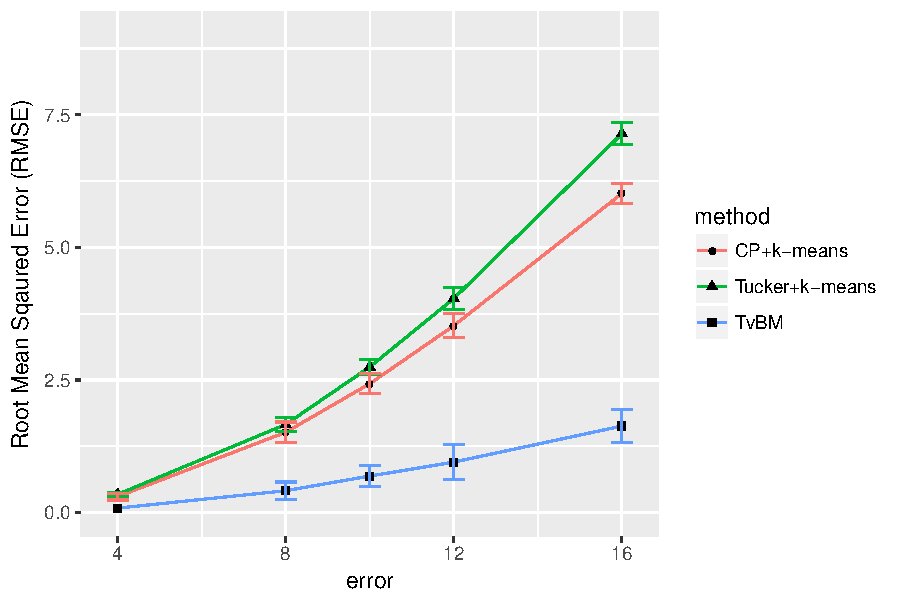
\includegraphics[width=.5\textwidth]{figures/sparse}
\caption{Sparse tensor}\label{fig:sparse}
\end{figure}

\begin{tabular}[ccc]
 "China"   "Cuba" "Poland"   "USSR" & UK/USA& 4
\end{tabular}

\begin{itemize}
\item 2 (Exports): reltreaties, booktranslation, relbooktranslations, relexports, exports3
\item 4 (Independence): "timesinceally"  "independence" 
\item 5 (NGO): relintergovorgs"          "relngo"   "intergovorgs3"        "ngoorgs3" 
\item 6 (edunvote)"treaties"      "conferences"   "weightedunvote" "unweightedunvote" "intergovorgs"              "ngo" 
\item 9 (tourist):"officialvisits"      "exportbooks"   "relexportbooks"          "tourism" "reltourism"         "tourism3"          "exports" "militaryalliance" 
 "commonbloc2" 

\end{itemize}



\end{appendices}
\end{document}
